\documentclass{article}

\title{Estimating Comparative Advantage in Improved Seed Adoption: Hybrid Maize in Ethiopia}

\usepackage{natbib}
\bibliographystyle{rusnat}

\usepackage{graphics}

\usepackage[margin=1in]{geometry}
\usepackage{setspace}
\doublespacing


\begin{document}

\maketitle

\section{Introduction}

Food security is a major challenge in many East African countries-- Ethiopia is no exception, having historically struggled to provide an adequate and reliable food supply \citep{Ramakrishna2002-hv, Jaleta2018-oj}. Since the drought of 1984, Ethiopia has become increasingly reliant on maize. Despite numerous technological breakthroughs in maize germplasm with increased yields and drought tolerance, adoption of improved seed has remained a challenge. There is a broad literature on why sub-Saharan farmers continue to use traditional farming techniques when more modern, higher-return agricultural technologies are available. Several answers have been proposed to explain this puzzle. These include imperfections in credit markets \citep{Croppenstedt2003-pq}, property rights \citep{Place2000-el}, social learning \citep{Conley2010-ue,Foster1995-bz,Munshi2004-og}, lack of commitment devices \cite{Duflo2009-iv}, and high transportation costs that increase the cost of agricultural inputs \citep{Byerlee2013-qk}. This issue is becoming more important as even current varieties of improved seed are over 20 years old and their effectiveness in terms of yield improvement and disease resistance is waning \citep{Abate2015-rj}. 

Adoption of a technology involves several dimensions such as market integration, access to supplementary inputs like fertilizer, as well agro-ecological considerations such as climate, altitude and soil quality. Ignoring the heterogeneity of these factors can hide the true impact of adoption, as different sub-populations may be impacted by the same technology in different, and even opposite ways. One way to tackle this problem, proposed by \citep{Suri2011-oi}, centers around quantifying the comparative advantage of a household to adopting improved seed varieties. Even when average returns are high, farmers may face heterogeneous returns based on their own, unobservable, comparative advantage in adopting new technologies. Using a correlated random coefficient model, Suri’s seminal paper finds that farmers’ lack of adoption is driven by insufficient net benefits to the technology stemming from poor infrastructure. Similar work in Ethiopia on improved chickpea varieties suggests that the economic returns to adoption plays a major role in the decision to adopt \citep{Michler2018-wk}. In our paper, we build on that literature by investigating hybrid maize seed adoption in Ethiopia, focusing on how heterogeneous returns are also driven by climate and how this can affect dis-adoption decisions.

We will explore how the role of heterogeneity in a household’s comparative advantage explains differences in the returns to adoption, and what drives those differences. Our objectives center around four main questions: (1) does adoption of improved seed take place where the net benefits of adoption is highest? (2) How do adaptation strategies such as water storage, and irrigation augment a household’s comparative advantage in adoption?, (3) what are the drivers of dis-adoption of improved maize seed? and (4) is it possible to extend the methodology in \citep{Tjernstrom_Emilia_Dalia_Ghanem_Oscar_Barriga_Cabanillas_Travis_J_Lybbert_Jeffrey_D_Michler_and_Aleksandr_Michuda2020-bc} by including time-varying characteristics to the Group Random Coefficients (GRC) model?

\section{Context}

Evidence has shown that the adoption of improved seed leads to increases in agricultural yields \citep{Carter2014-fm}, food security \citep{Shiferaw2014-op} and poverty reduction \citep{Minten2008-tj}. Despite such positive impacts, the low adoption levels of improved seeds varieties in Sub-Saharan Africa remains a puzzle. Multiple explanations have been proposed for observed adoption rates, including the type of technology promotion mechanisms used by governments, NGO’s, and businesses, the characteristics of the improved seeds and their adaptation to specific agro-climatic environments \citep{Bird2020-nt}, as well as growing conditions, such as the type of soil, input use, and other farmer characteristics \citep{Munshi2004-og}. Specifically, extension services and on-farm field trials, seed variety characteristics and rainfall have been found to be crucial to the adoption of improved maize in Tanzania \citep{Kaliba2000-jh}. In Ethiopia, labor, fertilizer use, farmers’ experience with extension packages, rainfall suitability and prices have been shown to increase the opportunity cost of not adopting improved wheat varieties \citep{Wale2006-bv}. Market access and the accessibility of extension services are also critical in the adoption of improved chickpea varieties in Ethiopia \citep{Verkaart2019-ol}. Other important determinants of heterogeneous effects include risk aversion \citep{Holden2016-vy}, farm size \citep{Ghimire2015-bd}, and credit constraints \citep{Simtowe2008-jn,Balana2020-hx}. The consensus in this literature is that the success of improved varieties depends on a range of factors that need to be better understood. Success of improved seeds should be accompanied by complementary conditions and inputs that would allow the full potential of these varieties to be realized.
A different branch of the literature provides an alternative explanation for such low adoption rates, focusing on heterogeneous potential returns to adoption \citep{Suri2011-oi}. This literature suggests that even if returns to adoption are high, farmers may fail to adopt if they face low comparative advantage to adoption. Other methods used in the literature fail to account for this heterogeneity, admitting only the presence of time-constant and/or time-varying unobserved heterogeneities (depending on the data structure) for identification purposes \citep{Kassie2018-xn,Falco2011-rt}. These methods ignore the possibility of a farmer’s comparative advantage of using an improved technology over a traditional one as playing a central role in their adoption decision. We rely on Suri’s method and its extension in \citep{Tjernstrom_Emilia_Dalia_Ghanem_Oscar_Barriga_Cabanillas_Travis_J_Lybbert_Jeffrey_D_Michler_and_Aleksandr_Michuda2020-bc} to account for such heterogeneous comparative advantages and evaluate how these are explained by climatic conditions. In Ethiopia, rainfall deviations from historical averages are found to be the main driver of heterogeneous effects for adopting agronomic packages \citep{Marenya2020-kb}. In Malawi, exposure to past droughts is found to increase the adoption of drought-tolerant maize among farmers that also receive subsidies \citep{Katengeza2019-af} and the dis-adoption of traditional local maize \citep{Holden2016-vy}. We will contribute to this literature by considering historical climate averages on the suitability of improved varieties to understand whether adoption is indeed realized where its potential is highest. Moreover, we will contribute to the understanding of how water conservation innovations and irrigation mitigate the effects of droughts on the potential of improved seeds.

\section{Data}

The current study uses the Ethiopia Socioeconomic Survey (ESS), a part of the Agricultural Sample Survey (AgSS), a survey 
designed to obtain production estimates for the major crops. It was conducted in collaboration with the Central Statistics Agency of Ethiopia, the World Bank and CGIAR (Consortium of International Agricultural Research Centers) \citep{kosmowski2020shining}. The ESS is meant to be representative of the most populous regions of the country. The ESS contains several questionnaires targeted at getting an understanding of the state of agriculture. This includes a survey that is conducted post-planting and then post-harvest. These surveys are more important to our analysis as it gives a close look to inputs used in agriculture, the types of seeds used (in various levels of detail) and yields collected post-harvest. There were significant differences between the analysis carried out in ESS 1-3 and the most recent, ESS4. Most notably, the ESS4 is no longer a panel dataset made up of the households of ESS 1-3, but it includes important information on the DNA fingerprinting of seed type and misclassification rates. This is important information as the first three waves of ESS only included self-reported hybrid maize status. Since our estimation strategy requires a balanced panel dataset of maize growers, our main analysis will include the first three waves of the ESS. We use the fourth wave later for robustness and validation.

Figure \ref{map:regions} shows the spatial distribution of the locations of the our households of study. As previously mentioned these are households that grow either improved or conventional maize and that are observed for all three rounds of the survey. Most households come from the northwest region of the

\begin{figure}
    \centering
    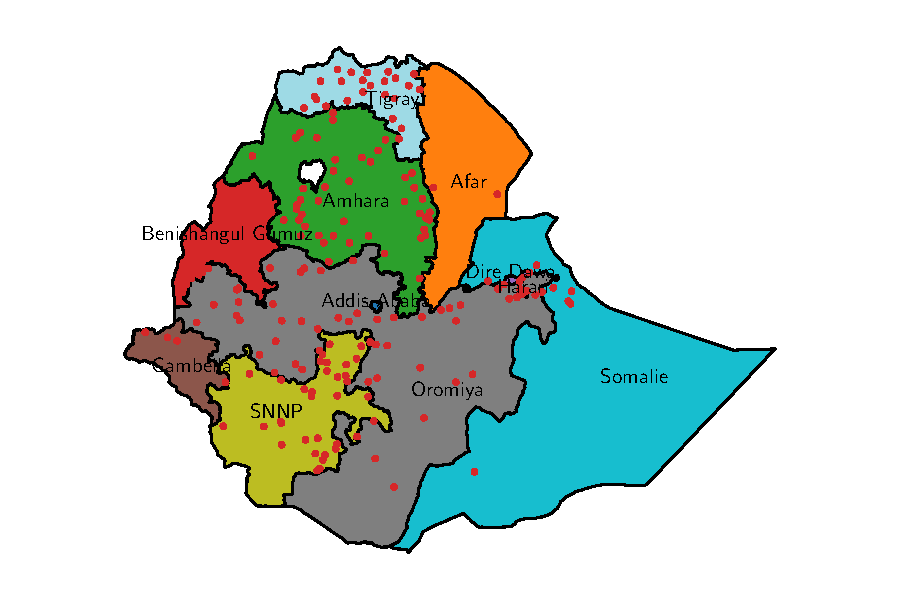
\includegraphics{results/figures/map_hhids.pdf}
    \caption{Spatial Distribution of Households Surveyed}
    \label{map:regions}
\end{figure}

Table \ref{tbl:summary} shows a set of the summary statistics for the sample of house

\section{Estimation Strategy}

Methods 

Our base analysis will be inspired by the work of \citep{Suri2011-oi}. This estimation framework imposes a parametric relationship between farmers' absolute advantage (i.e., the component of productivity that is independent of technology) and their comparative advantage (i.e., their relative productivity of adopting the improved technology over not adopting). This method seeks to estimate the following equation:

$$
yit=+ hit + i+ihit + i+it
$$

where y is yields or profits for household i at time t, h is an indicator for adoption,  is a household’s absolute advantage,  is a household’s comparative advantage and  describes the gains to adopting, relative to a household’s comparative advantage. This framework provides an advantage over other methods \citep{Wooldridge1997-xj,Heckman1998-pt}. Firstly, identification does not rely on the existence of a valid instrumental variable. Instead, identification comes from a linear projection of an individual's returns to adoption onto the observed history of their adoption, an approach similar to the correlated random effects (CRE) method in \citep{Chamberlain1984-uk}. Secondly, it disentangles a household’s absolute advantage when taking part in agriculture and its comparative advantage in adopting. This is crucial in understanding the adoption decision as it is not dependent on a household’s agricultural ability, but on the gains from taking it up. We and co-authors developed this further in \citep{Tjernstrom_Emilia_Dalia_Ghanem_Oscar_Barriga_Cabanillas_Travis_J_Lybbert_Jeffrey_D_Michler_and_Aleksandr_Michuda2020-bc} by proposing a more flexible and tractable approach using a group random coefficient strategy that draws on recent developments in the nonparametric panel identification literature. Our strategy has a clear economic interpretation and can elucidate potential identification concerns of the CRC model to the practitioner. It is also more easily extended to multiple time periods and new levels of heterogeneity than the CRC approach.

Estimating equation 1 will allow us  to analyze the distribution of the gains to adoption and to create a distribution of heterogeneous returns. We will investigate whether comparative advantage is driven by two key policy relevant factors: water conservation strategies and deviation from historical climate averages. The first will elucidate if adaptation strategies in water management are associated with higher levels of gains to adoption. The second will seek to understand whether households are adapting to climate change through their adoption decisions. This will require the extension of the method developed in \citep{Tjernstrom_Emilia_Dalia_Ghanem_Oscar_Barriga_Cabanillas_Travis_J_Lybbert_Jeffrey_D_Michler_and_Aleksandr_Michuda2020-bc}, by allowing for time-varying characteristics in the identification of comparative advantage.

Implications 

Our work has far-reaching policy implications. The adoption and impact of agricultural technologies is inherently heterogeneous. Our methodology incorporates that from the outset, allowing us to investigate whether synergies between seed adoption and water conservation strategies interact; a key component to understanding how investment into such projects translates to economic returns. Moreover, our research informs on not only the adoption but also dis-adoption decisions of technologies as well. In this sense, we provide valuable information to policymakers on how to better target seed marketing or infrastructure to help agricultural households improve their livelihoods

\section{Results}

\section{Conclusion}

\bibliography{references}


\end{document}